\chapter{Desenvolvimento da aplicação AutoForm}
% ---
Neste capitulo é apresentado o desenvolvimento do projeto, onde são apresentados, a arquitetura do sistema, o processo de produção, e a implementação do sistema.

\section{Processo de produção}
O projeto teve sua fase inicial, após o 1º encontro com o cliente Tiago Costa e o coorientador Márcio Lemos no \textit{campus} Osório do IFRS, na reunião foi demonstrada a necessidade pela BM RS de uma aplicação que pudesse ser utilizada para auxiliar no processo de registro do AEL no SIGMA, a fim de agilizar o processo de preenchimento e automatizar a geração do arquivo, bem como resolver outras dificuldades encontradas pelos operadores.
Após a definição de contexto do AEL por parte da BM RS, foi realizado um estudo sobre o assunto, para que fosse possível entender o problema e propor uma solução viável e eficaz.
Sendo demonstrado na  \autoref{fig:diagramaBPMN} o fluxo desse processo e como a aplicação web AutoForm iria atuar.

\begin{figure}[H]
    \caption{\label{fig:diagramaBPMN}Diagrama de processo BPMN}
    \begin{center}
        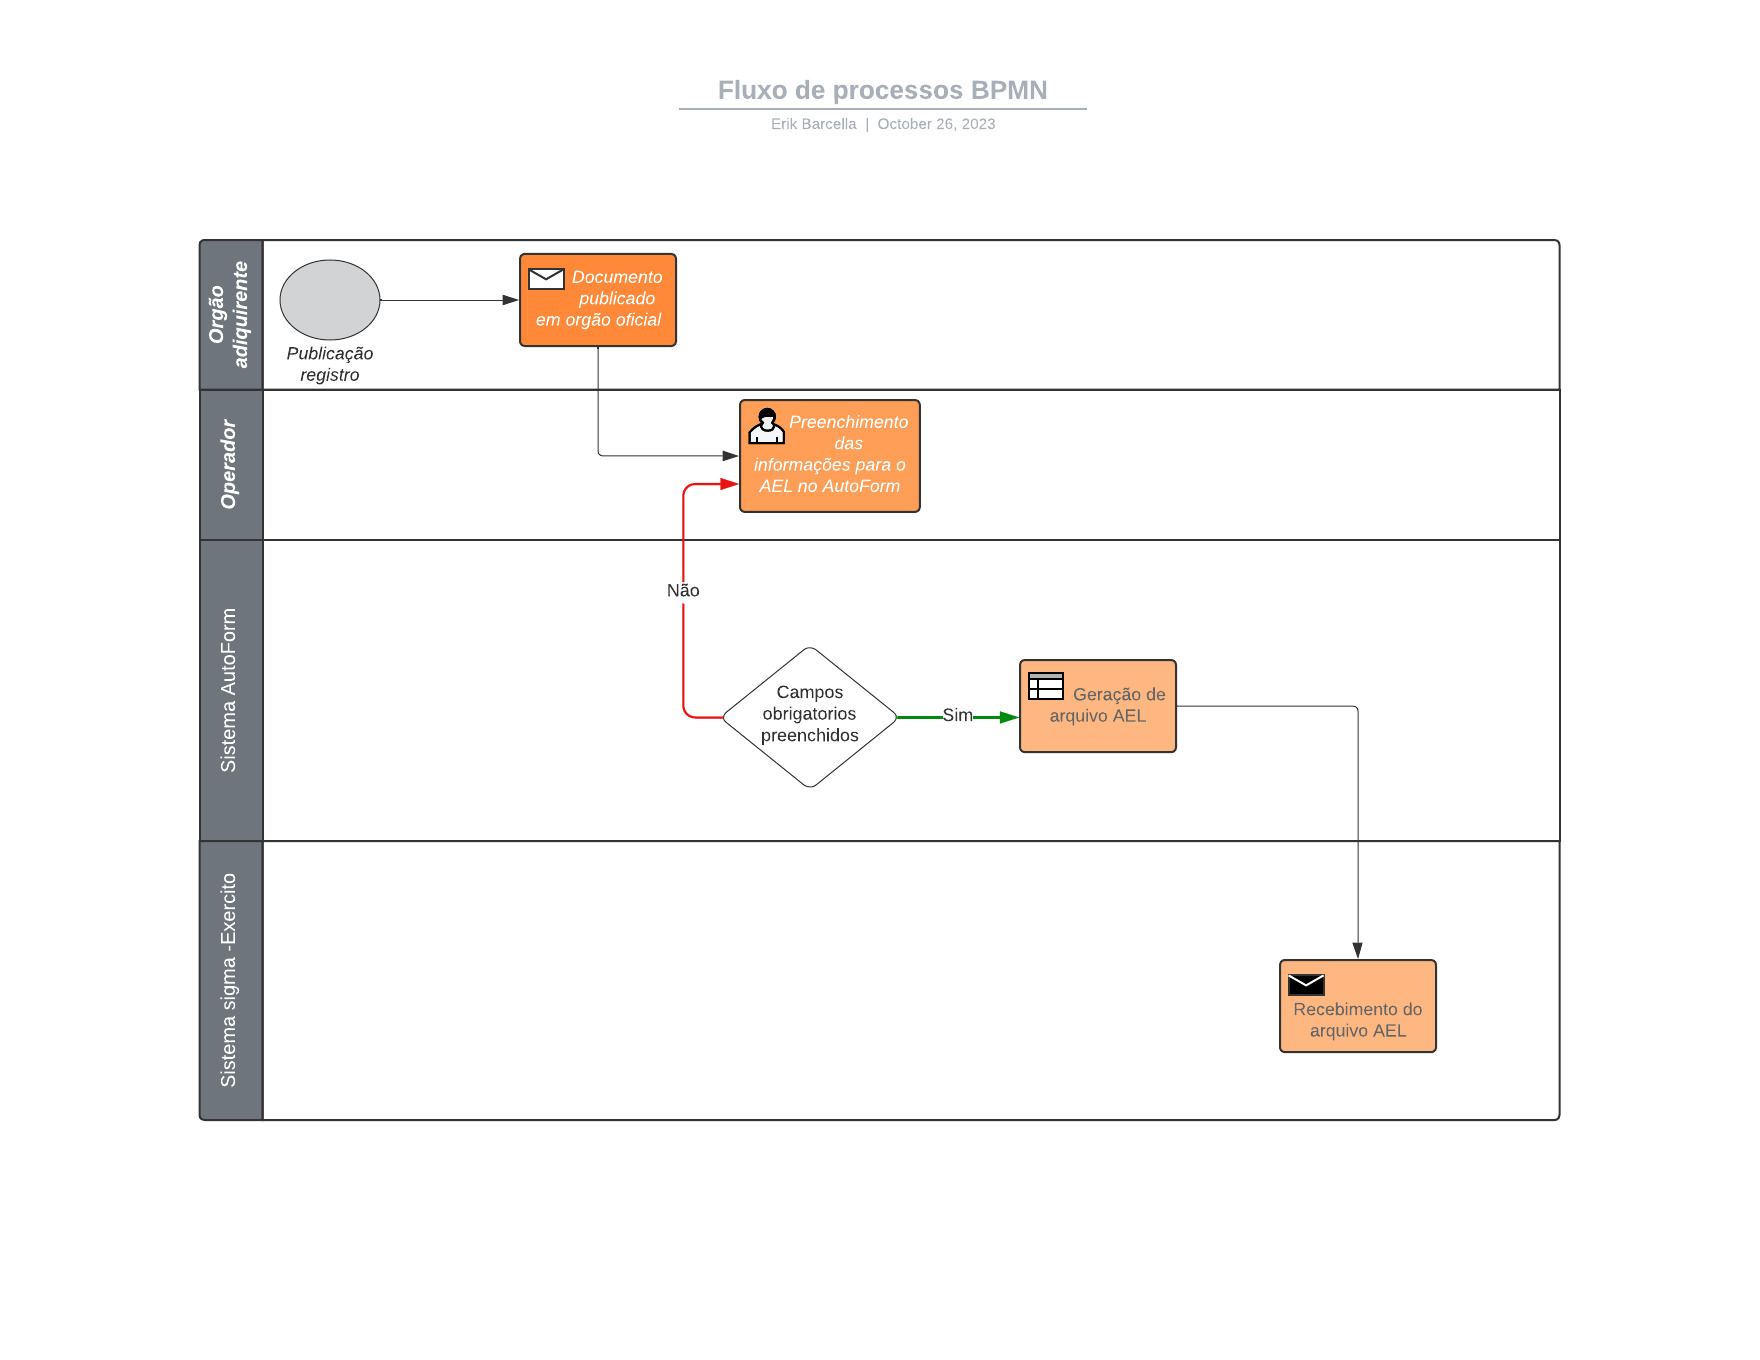
\includegraphics[scale=0.50]{imagens/FluxodeprocessoBPMN.jpeg}
    \end{center}
    \legend{Fonte: Autor}
\end{figure}

Com a elicitação dos requisitos concluída, ocorreu a prototipação das telas da aplicação, utilizando a ferramenta de \textit{design de interface } de usuário \citeonline{figma}, a fim de validar se o visual e o fluxo da aplicação iriam atender o proposito da instituição.


\subsection{Tecnologias}\label{sec:tecnologias}
Após a validação do protótipo, foi realizada a escolha das tecnologias que seriam utilizadas no desenvolvimento da aplicação, sendo elas o \textit{framework} \citeonline{ReactMet54}, para o desenvolvimento \textit{frontend}, e o \textit{framework} NodeJS \citeonline{Nodejs} para o desenvolvimento do \textit{backend} da aplicação web, juntamente com o banco de dados não relacional \citeonline{MongoDBA45:online}, para o armazenamento dos dados.

Com as tecnologias definidas, foi realizado o desenvolvimento da aplicação web e hospedado em um servidor, para que fosse possível realizar os testes e validações com o cliente, e assim, realizar as correções necessárias. 

Portanto após a primeira versão da aplicação estar disponível na \textit{internet} as adaptações necessárias e atualizações eram organizadas e relatadas mediante troca de mensagens com o cliente.

Para permitir que fosse possível realizar atualizações em produção na aplicação foi utilizada a ferramenta \citeonline{git}, juntamente com a plataforma de hospedagem de código fonte \citeonline{github}, para que fosse possível realizar o controle de versões e o versionamento do código fonte da aplicação, garantindo sempre uma versão estável e disponível em produção, enquanto era viável desenvolver paralelamente novas funcionalidades e valida-las com o cliente.

\subsection{Arquitetura da aplicação}
Nesta seção será abordado a visão de como foi projetado a estrutura do sistema que é composto por uma aplicação web, e uma API.

A Arquitetura \textit{MVC} foi a escolhida para a estruturação do sistema, ficando então dispostas as tecnologias mencionadas na \autoref{sec:tecnologias} da seguinte maneira ilustrada pela  \autoref{fig:diagramstacks}.

Toda comunicação entre a aplicação web e a API é realizada através de requisições HTTP, onde a aplicação web realiza requisições para a API, e a API responde com os dados solicitados, caso necessário a API busca as informações no banco de dados e retorna para a aplicação web.

As requisições e respostas seguem o padrão REST, onde cada requisição possui um método HTTP, e um \textit{endpoint} que é a URL que identifica o recurso que está sendo solicitado. A resposta da requisição é um JSON, que contém os dados solicitados.

\begin{figure}[H]
    \caption{\label{fig:diagramstacks}Disposição das tecnologias na arquitetura MVC}
    \begin{center}
        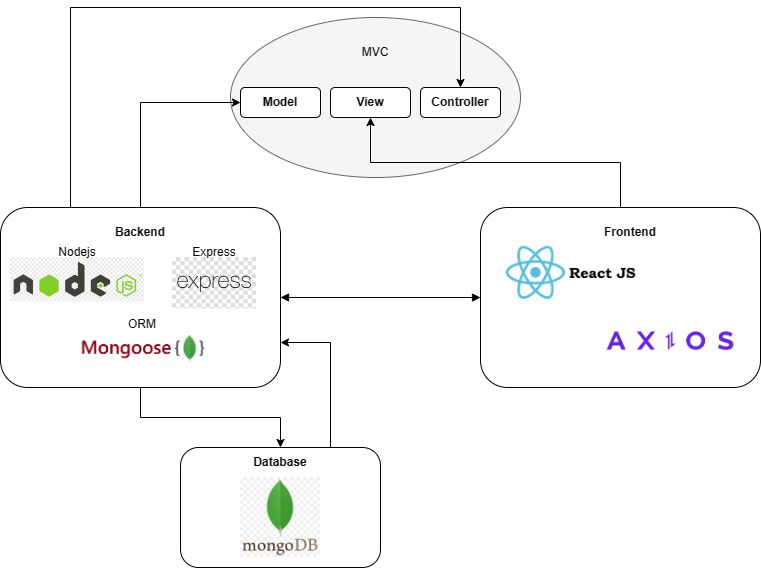
\includegraphics[scale=0.5]{imagens/diagrama.png}
    \end{center}
    \legend{Fonte: Autor}
\end{figure}

Atuando na camada de modelo da aplicação, o banco de dados é responsável por armazenar os dados da aplicação e foi construido utilizando dois modelos principais para armazenamento não estruturado, o modelo evidenciado na \autoref{fig:diagrama-user} é utilizado para representar as informações referente aos usuários da aplicação.

Enquanto o modelo representado na \autoref{fig:diagrama-armas} representa as informações referente as armas.


\begin{figure}[H]
    \caption{\label{fig:diagrama-user}Diagrama da estrutura de usúario}
    \begin{center}
        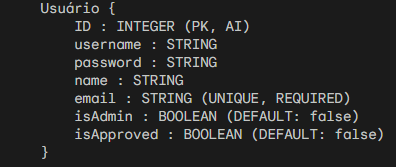
\includegraphics[scale=1]{imagens/diagramaUser.png}
    \end{center}
    \legend{Fonte: Autor}
\end{figure}

\begin{figure}[H]
    \caption{\label{fig:diagrama-armas}Diagrama da estrutura de armas}
    \begin{center}
        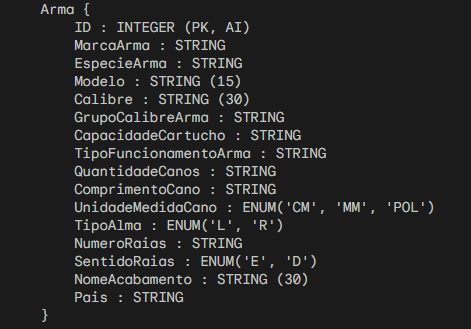
\includegraphics[scale=0.82]{imagens/diagramaArma.png}
    \end{center}
    \legend{Fonte: Autor}
\end{figure}






\subsection{Aplicação Web AutoForm}

\subsection{Autenticação}

A página para acessar a aplicação \autoref{fig:tela-login} e a página de registro \autoref{fig:tela-registro} são de acesso público, portanto podem ser visualizadas sem a necessidade de autenticação, já para acessar as demais páginas é necessário realizar o login.

A estratégia empregada para o acesso consiste na autenticação por meio de token JWT. O usuário realiza o login, fornecendo sua identificação de funcionário e senha. Essas informações são então encaminhadas para a API por meio de uma requisição POST. 
A API valida no banco de dados a existência de um usuário com os dados fornecidos. 
Se a validação for bem-sucedida, a API gera um token de acesso e o retorna como resposta. Posteriormente, a aplicação decodifica o token recebido, que contém as informações do usuário no \textit{payload}, e armazena os dados de identificação no navegador da pessoa que solicitou o acesso.

A cada requisição posterior para outros \textit{endpoints} que a aplicação realize para a API, o token é enviado no cabeçalho da requisição. A API irá validar somente o token, e caso seja válido retorna os dados solicitados.

\subsection{Página de login}
Está página é responsável por realizar a autenticação do usuário, e para isso é necessário informar a identificação de funcionário e a senha. Caso o usuário não possua cadastro, é possível realizar o registro, clicando no botão "Registrar-se", que redireciona para a página de registro.

\begin{figure}[htb]
    \caption{\label{fig:tela-login}Autoform - Página de login}
    \begin{center}
        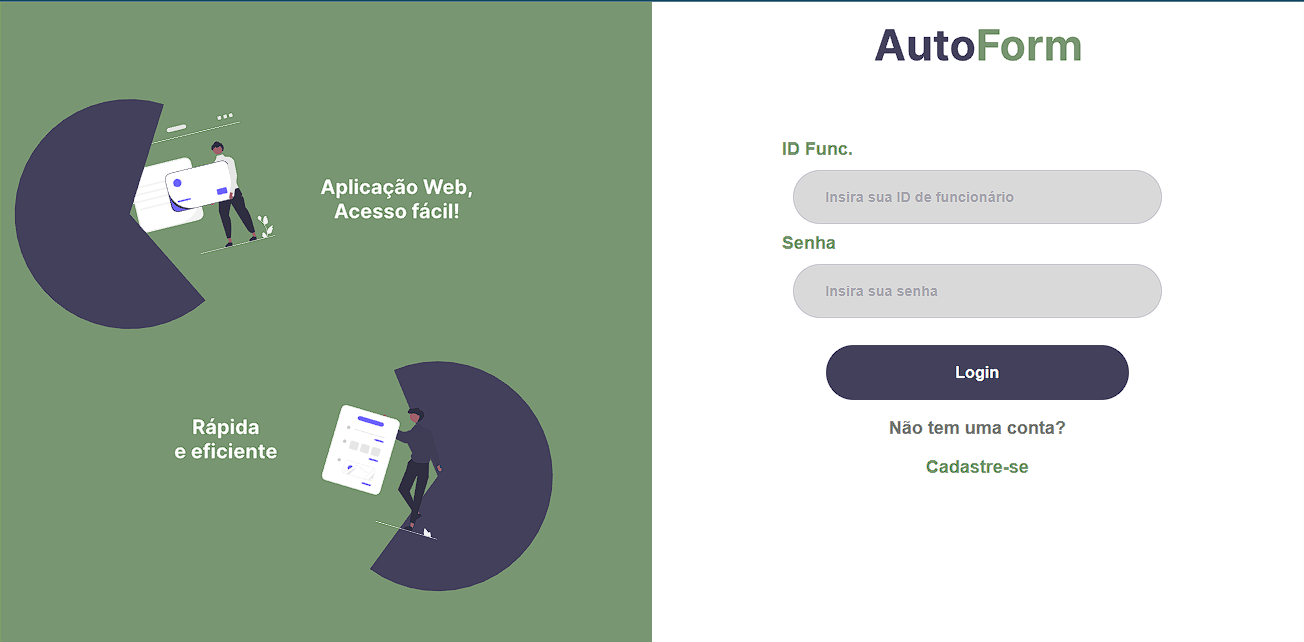
\includegraphics[scale=0.45]{imagens/login-autoform.png}
    \end{center}
    \legend{Fonte: Autor}
\end{figure}

 Se, por acaso, a validação no banco de dados não for bem-sucedida, a API emite uma resposta personalizada, indicando a natureza específica do impedimento.

Em um cenário em que a Identificação de Funcionário ou a senha fornecida não corresponde aos registros existentes, um alerta sutil é gerado, informando ao usuário sobre a disparidade. Este mecanismo proativo visa aprimorar a eficiência da correção do erro, direcionando o usuário a revisar e corrigir suas credenciais antes de prosseguir com a autenticação.
Ademais, é importante ressaltar que, em situações extremas, como indisponibilidade temporária do serviço de autenticação, o usuário é informado sobre a impossibilidade de acesso, e orientado a tentar novamente mais tarde.

\subsection{Página de registro}
A página de registro \autoref{fig:tela-registro} é responsável por realizar o cadastro de novos usuários, e para isso é necessário informar o email, a identificação de funcionário, a senha, e a confirmação da senha. E em caso de sucesso será retornada uma mensagem informando que o registro foi efetuado com sucesso.

\begin{figure}[htb]
    \caption{\label{fig:tela-registro}Autoform - Página de registros}
    \begin{center}
        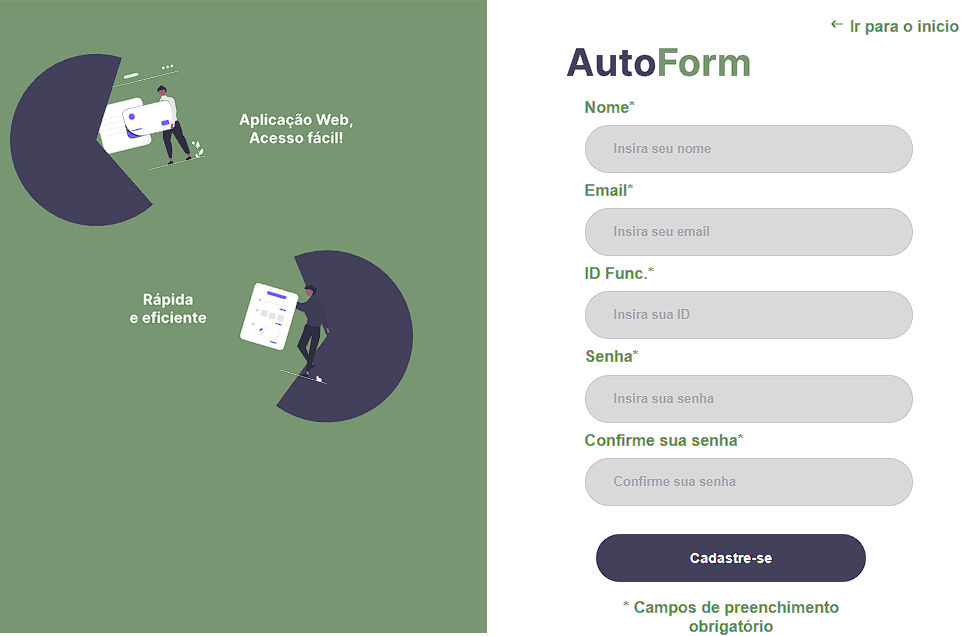
\includegraphics[scale=0.6]{imagens/registro-autoform.png}   
     \end{center}
    \legend{Fonte: Autor}
\end{figure}
Caso a identificação de funcionário já esteja cadastrada, será retornada uma mensagem informando que a identificação de funcionário já está cadastrada.
Em caso de não conformidade da senha com a confirmação da senha, será retornada uma mensagem informando que as senhas não conferem.

\subsection{Página inicial}
Na \autoref{fig:tela-home-inicio} é exibido a tela inicial da aplicação, a qual o usuário é direcionado assim que realiza o login, e nela é possível visualizar no menu lateral as opções disponíveis de criação de AEL, cadastros, usuários e sair da aplicação.

\begin{figure}[H]
    \caption{\label{fig:tela-home-inicio}Autoform - Página inicial home}
    \begin{center}
        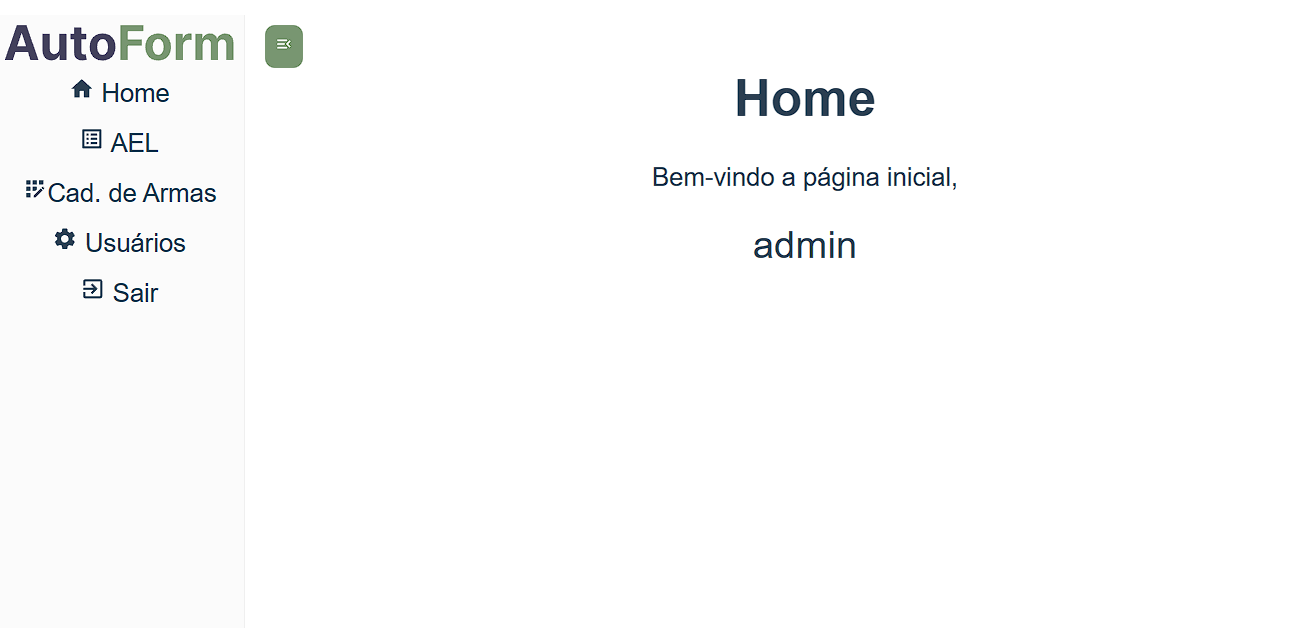
\includegraphics[scale=0.35]{imagens/home-autoform.png}
    \end{center}
    \legend{Fonte: Autor}
\end{figure}

\subsection{Página de criação de AEL}
A página de criação de AEL, \autoref{fig:tela-ael1}, é responsável por realizar a criação de um registro e geração do AEL, sendo necessário informar os campos obrigatórios que constam no \autoref{sec:anexoA2} e \autoref{sec:anexoA3}.

Cada registro é salvo no \textit{local storage} do navegador do usuário com todas informações preenchidas no formulário, para posterior geração do arquivo. 

Essa estratégia de armazenamento temporário foi adotada visando manter a integridade e a segurança das informações caso o usuário perca a conexão com a internet ou por algum outro motivo a aplicação do navegador seja encerrada, o que acarretaria na perca de todos os registros já digitados, utilizando essa abordagem é possível resgatar da memoria do navegador todos os registros salvos temporariamente para geração do AEL, sem necessidade de armazenar no banco de dados ou enviar pela rede informações sensíveis como CPF entre outros. 
\begin{figure}[htb]
    \caption{\label{fig:tela-ael1}Autoform - Página de criação do AEL}
    \begin{center}
        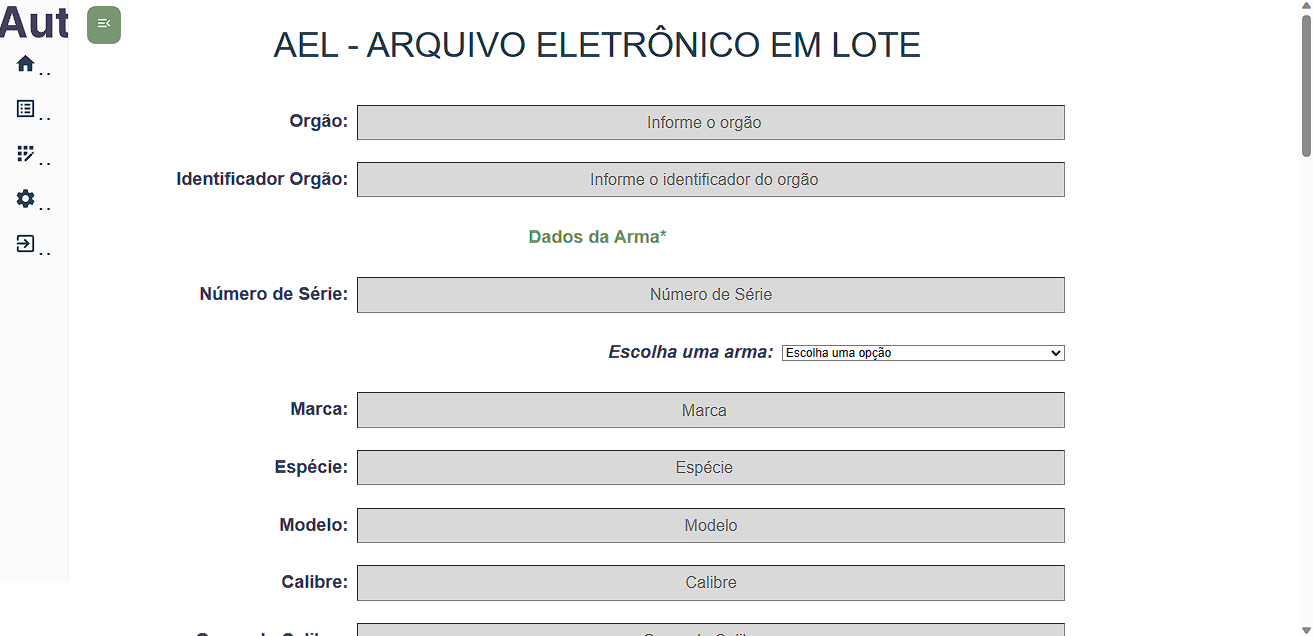
\includegraphics[scale=0.45]{imagens/autoform-ael-gerar.png}
    \end{center}
    \legend{Fonte: Autor}
\end{figure}

\subsection{Página de criação de AEL com opção de autopreenchimento}
Na \autoref{fig:tela-ael-selecao} podemos visualizar um input que exibe uma lista com as armas cadastradas, facilitando o preenchimento de diversos campos do formulário,
pois permite ao usuário selecionar uma arma previamente cadastrada, e os respectivos campos do formulário serão preenchidos automaticamente.

\begin{figure}[H]
    \caption{\label{fig:tela-ael-selecao}Autoform - Página de criação do AEL com opção para selecionar}
    \begin{center}
        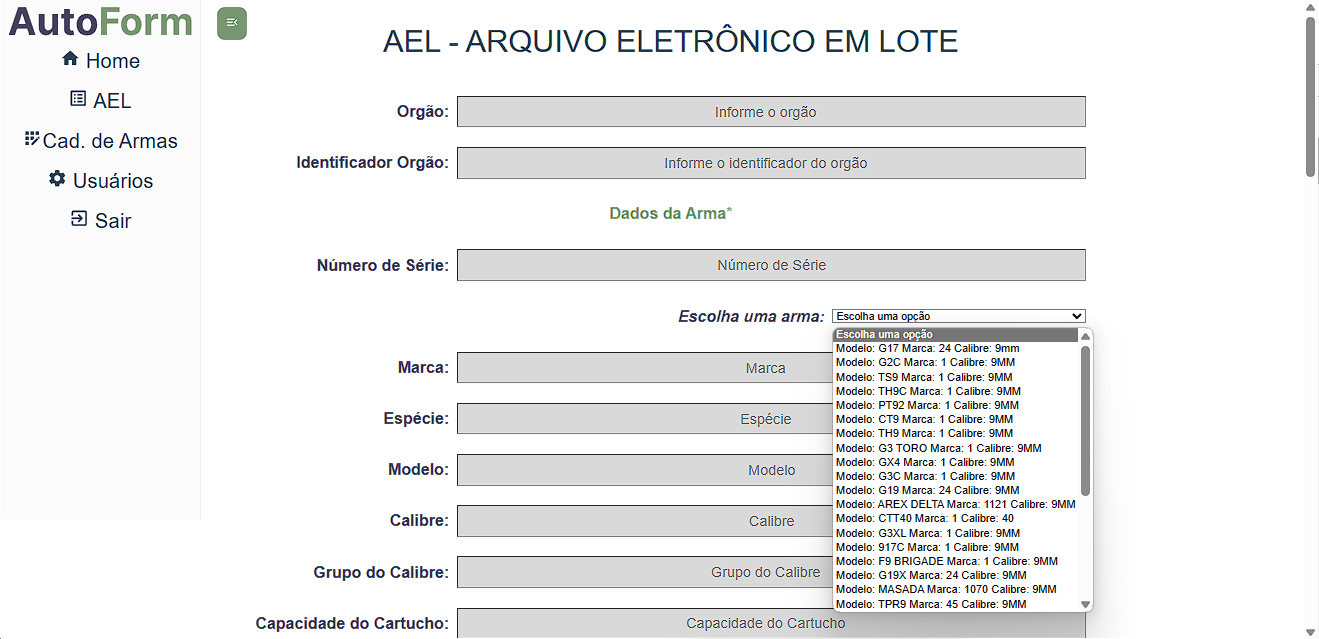
\includegraphics[scale=0.45]{imagens/autoform-ael-selecao.png}
    \end{center}
    \legend{Fonte: Autor}
\end{figure}

\begin{figure}[H]
    \caption{\label{fig:tela-ael2}Autoform - Página de criação do AEL -2}
    \begin{center}
        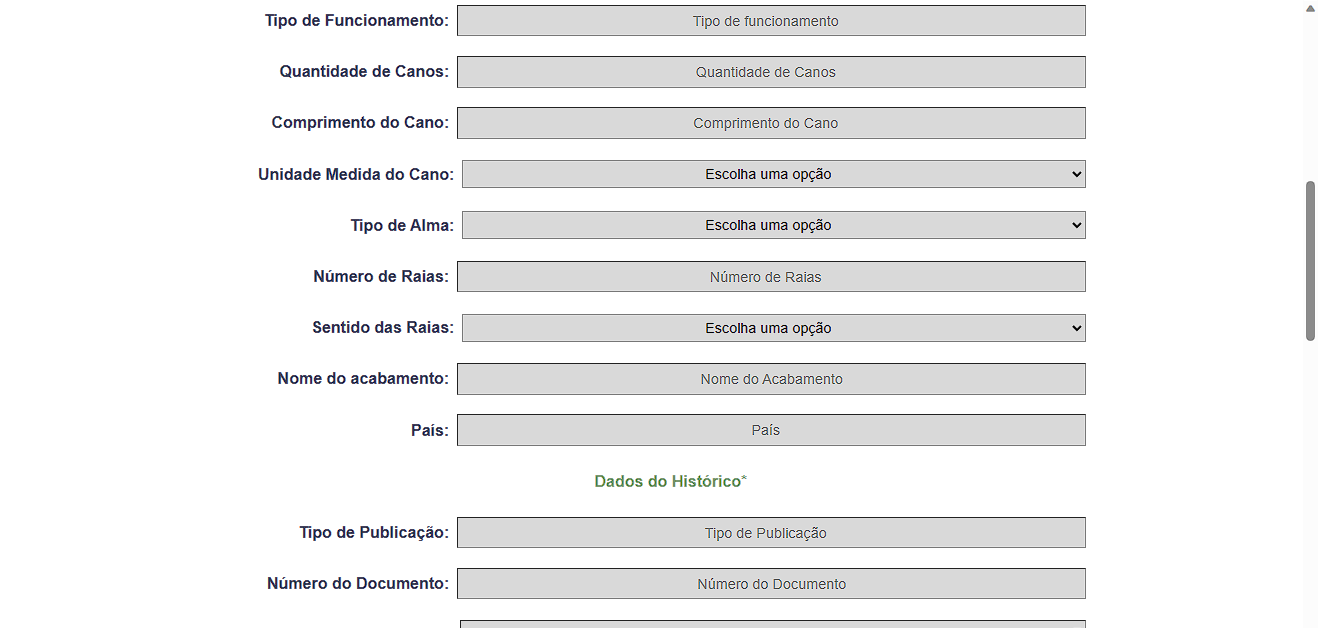
\includegraphics[scale=0.45]{imagens/autoform-ael-gerar2.png}
    \end{center}
    \legend{Fonte: Autor}
\end{figure}
\begin{figure}[H]
    \caption{\label{fig:tela-ael3}Autoform - Página de criação do AEL-3}
    \begin{center}
        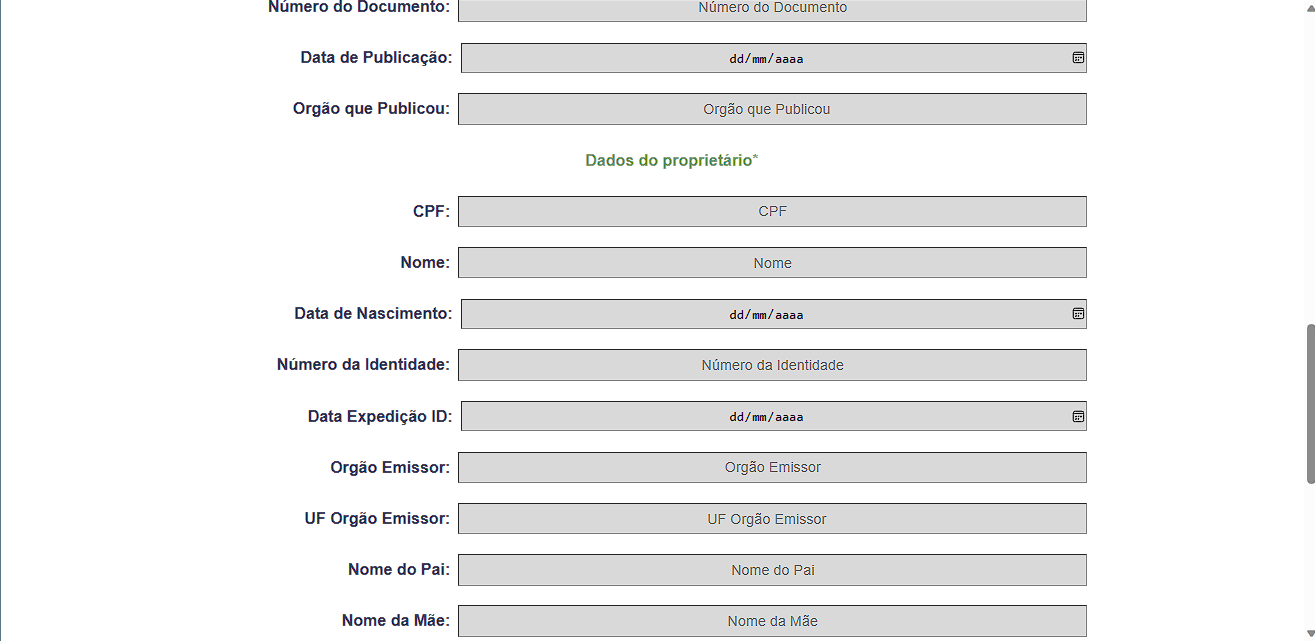
\includegraphics[scale=0.45]{imagens/autoform-ael-gerar3.png}
    \end{center}
    \legend{Fonte: Autor}
\end{figure}

\begin{figure}[H]
    \caption{\label{fig:tela-ael4}Autoform - Página de criação do AEL-4}
    \begin{center}
        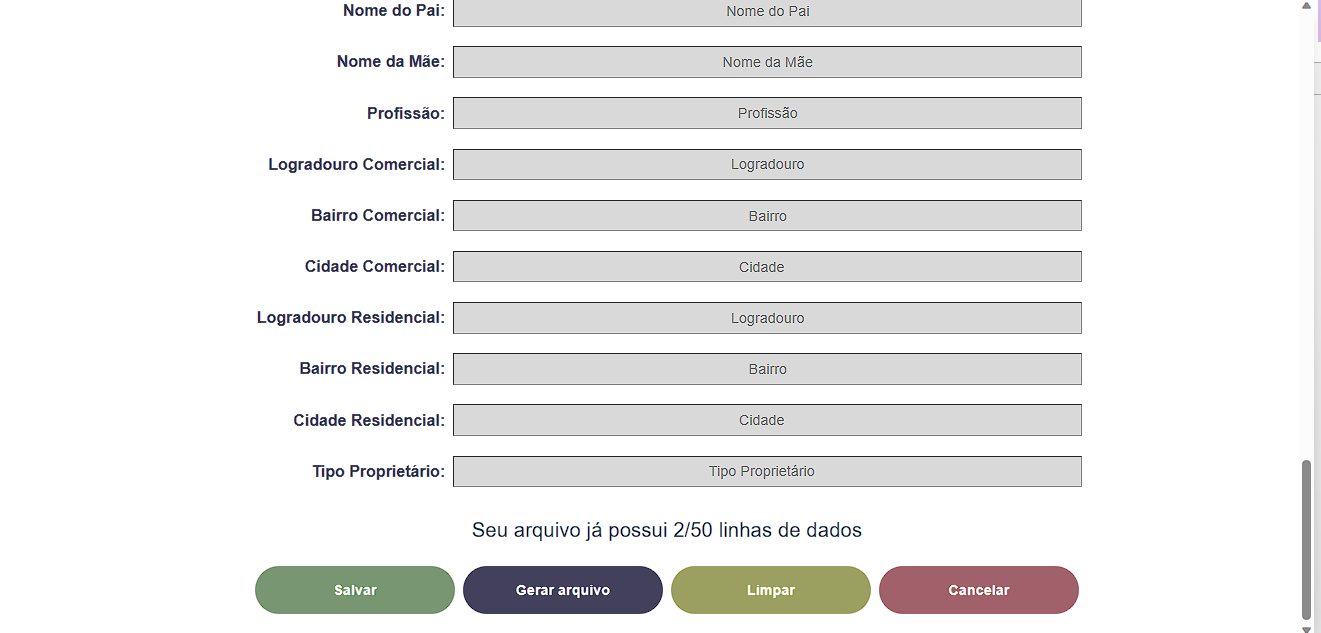
\includegraphics[scale=0.45]{imagens/autoform-ael-gerar4.png}
    \end{center}
    \legend{Fonte: Autor}
\end{figure}

Telas do formulário web para geração do AEL

Os botões da \autoref{fig:tela-ael4} tem as seguintes funcionalidades:
\begin{itemize}
    \item Salvar: Verifica se todos os campos obrigatórios foram preenchidos, e caso estejam preenchidos, salva o registro no \textit{local storage} do navegador.
    \item Gerar Arquivo: Com base nos registros salvos no \textit{local storage}, a aplicação realiza a normalização das informações de acordo com as regras específicas de indexação contidas no \autoref{sec:anexoA1} e \autoref{sec:anexoA4}.
     
    Após uma caixa de pergunta é exibida ao usuário solicitando o nome do AEL e gera automaticamente o arquivo com base no nome inserido, realizando o download do arquivo AEL para o navegador do usuário que solicitou o recurso. 
    \item Limpar: Este botão exibe uma mensagem perguntando ao usuário se deseja limpar Nº linhas de registros contidos no armazenamento local do navegador.  Após confirmada a ação os registros temporários são apagados. 
    Esta opção foi implementada para garantir que após gerar o arquivo o usuário possa apagar os registros antigos para inserir novos. E também como garantia de segurança, limpando todos os dados do armazenamento temporário para  que não fique nenhuma informação sensível salva no navegador do usuário.
    \item Cancelar: Esse botão tem como intuito apenas direcionar o usuário para a página inicial da aplicação a \autoref{fig:tela-home-inicio}, saindo da opção de criação de AEL sem acarretar na perca dos registros temporários já salvos.
\end{itemize}

\subsection{Exemplo de AEL gerado}
Exemplo da ação executada após selecionar o botão gerar arquivo, que tem como saída o arquivo AEL formatado.

\begin{figure}[H]
    \caption{\label{fig:tela-ael-gerado}Autoform - AEL gerado}
    \begin{center}
        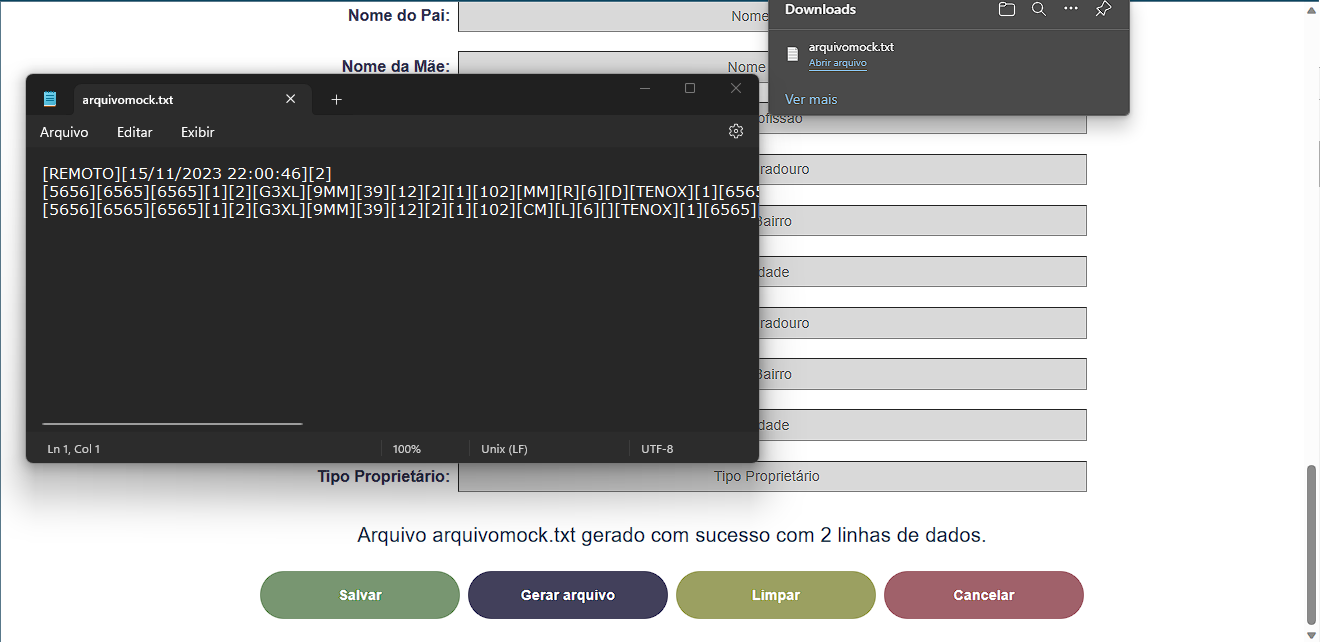
\includegraphics[scale=0.45]{imagens/autoform-ael-gerado.png}
    \end{center}
    \legend{Fonte: Autor}
\end{figure}


\subsection{Página de cadastros}
Na página de cadastros, \autoref{fig:tela-cadastros-armas}, é possível visualizar os cadastros de armas que são armazenadas no banco de dados, também é possível realizar uma pesquisa.
\begin{itemize}
    \item Pesquisar: Neste campo é possível realizar uma pesquisa por uma arma específica, e caso seja encontrado o registro, o mesmo será exibido na tabela.
    \item Alterar: Neste botão é possível alterar o registro de arma. Após a edição o registro é atualizado no banco de dados.
    \item Excluir: Neste botão é possível excluir o registro de arma. Após a exclusão o registro é removido do banco de dados.
    \item Cadastrar: Neste botão é possível cadastrar uma nova arma, onde será exibido um modal contendo um formulário para o usuário preencher os dados da arma. Após a confirmação o registro é inserido no banco de dados e uma mensagem de sucesso é exibida ao usuário.
\end{itemize}

\begin{figure}[H]
    \caption{\label{fig:tela-cadastros-armas}Autoform - Cadastros}
    \begin{center}
        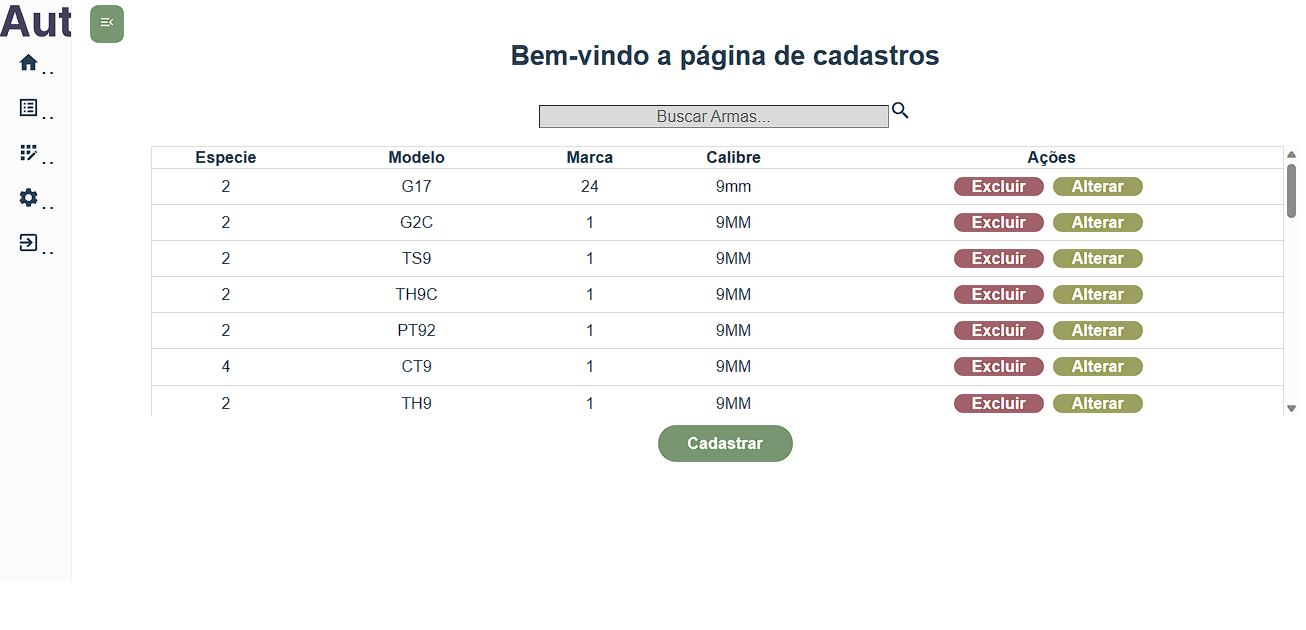
\includegraphics[scale=0.45]{imagens/autoform-cadastros.png}
    \end{center}
    \legend{Fonte: Autor}
\end{figure}


\subsection{Página de administração de usuários}
Esta página é acessível somente ao usuário com perfil de administrador.
Nela é exibido o nome, e-mail e status de autorização dos usúarios cadastrados.

Sendo possível realizar o gerenciamento destes através dos seguintes botões:
\begin{itemize}
    \item Pesquisar: Neste campo é possível realizar uma pesquisa por um usuário específico. Caso seja encontrado o registro, o mesmo será exibido na tabela.
    \item Excluir: Neste botão é possível excluir o registro de usuário. Após a confirmação de exclusão o registro é removido do banco de dados.
    \item Alterar senha: Neste botão é possível alterar a senha de usuário, onde será exibido um campo para o administrador informar a nova senha e após a confirmação. O registro é atualizado no banco de dados e uma mensagem de sucesso é exibida ao usuário.
    \item Autorizar: Ao utilizar esse botão é possível alterar o status do usuário para autorizado, liberando o acesso a aplicação. O registro é atualizado no banco de dados e uma mensagem de sucesso é exibida ao usuário.
    \item Bloquear: Ao utilizar esse botão é possível alterar o status do usuário para bloqueado, bloqueando o acesso a aplicação. O registro é atualizado no banco de dados e uma mensagem de sucesso é exibida ao usuário.
\end{itemize}

\begin{figure}[H]
    \caption{\label{fig:tela-configuracoes}Autoform - Administração de usuários}
    \begin{center}
        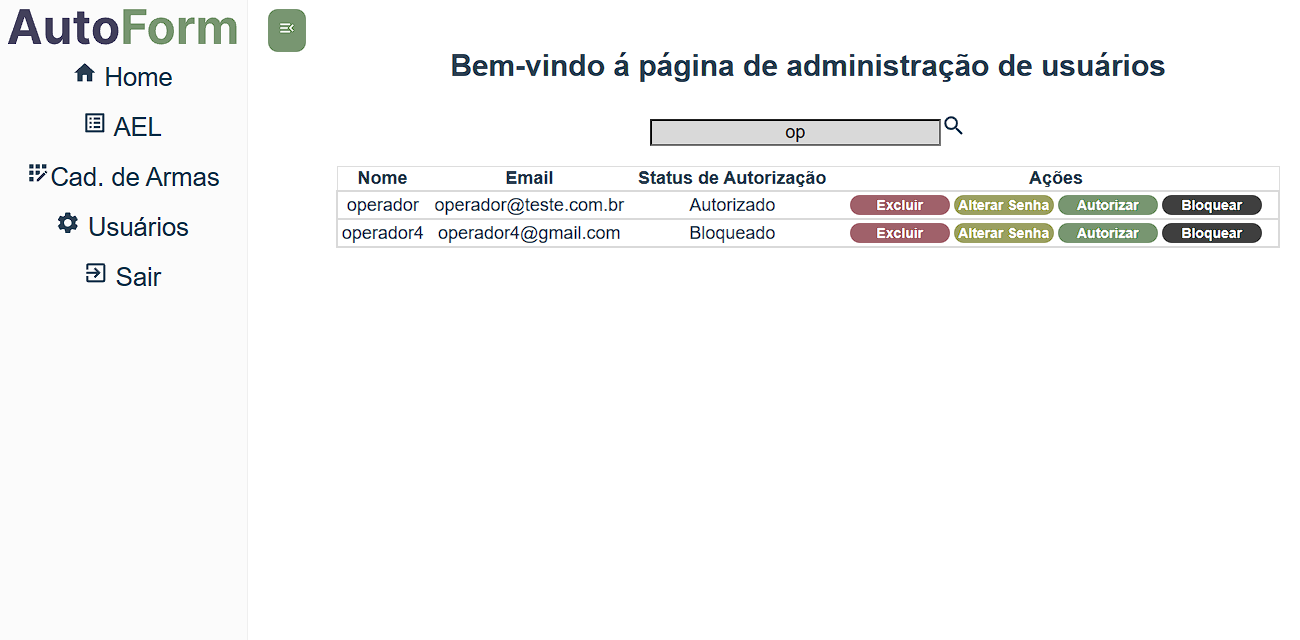
\includegraphics[scale=0.45]{imagens/autoform-configuracoes.png}
    \end{center}
    \legend{Fonte: Autor}
\end{figure}



% Este capítulo possui também exemplos de como inserir código no texto.
% % ---
% \section{Vestibulum ante ipsum primis in faucibus orci luctus et ultrices
% posuere cubilia Curae}
% % ---

% \lipsum[21-22]

% \section{Inserindo código no texto}

% Abaixo são apresentados exemplos de códigos inseridos no texto usando o pacote listings.

% %Inserindo código diretamente no texto
% \begin{lstlisting}[language=c, caption={Exemplo de código C}, upquote=true]
% #include <stdio.h>

% int main(int argc, const char * argv[]) {
% struct pessoa{
% char nome[20];
% char sobreNome[20];
% unsigned short idade;
% char cpf[15];
% }p1;
% //struct pessoa p1;

% printf("Digite o nome: ");
% scanf("%s",p1.nome);
% printf("Digite o sobrenome: ");
% scanf("%s",p1.sobreNome);
% printf("Digite a idade: ");
% scanf("%hu",&p1.idade);
% printf("Digite o CPF: ");
% scanf("%s",p1.cpf);

% printf("\nO nome da pessoa eh: %s", p1.nome);
% printf("\nO sobrenome da pessoa eh: %s", p1.sobreNome);
% printf("\nA idade da pessoa eh: %d", p1.idade);
% printf("\nO CPF da pessoa eh: %s\n", p1.cpf);
% }
% \end{lstlisting}

% \lipsum[1]

% %Ao invés de inserir código diretamente no texto, é recomendável importar um arquivo com o código

% %Importanto arquivo de código
% \lstinputlisting[language=Java,caption={Exemplo de código java}]{codigos/Minhaclasse.java}

% O método abaixo mostra a string mensagem recebida como parametro e retorna um inteiro digitado pelo usuario. Através de tratamento de exceções, o método executará até que o usuário digite um inteiro válido.

% %Para inserir apenas algumas linhas do arquivo
% \lstinputlisting[language=Java, caption={Método LerInteiro}, firstline=39, lastline=54]{codigos/Ferramentas.java}

% \lipsum[2-3]